% 2010 年重庆卷理科第 19 题：四棱锥 P-ABCD，底面 ABCD 为矩形，PA⊥底面，E 为棱 PB 的中点。
% 来源 PDF：普通高考/2010/2010重庆理.pdf，SHA-256 e981a8805207e307d0ec0d8ef50ac0e0cbf93eec9559a29fb88591b483ae0136。
% 原页：第 2 页（A3 三栏）第 1 栏上部，书页码 578。
% 重绘依据：按原页矢量路径逐段提取顶点位置（以 BC=4 为单位长）：
%   B(0,0)、C(4,0)、A(2,2)、D(6,2)、P(2,7.66)、E(1,3.83)，P 在 A 的正上方、E 为 PB 中点。
% 实线：BC、CD、CE、PB、PC、PD；虚线：PA、AB、AD、AC、AE、DE（与原页虚线段一一对应）。
% 原页在顶点 A 处画一个小叉表示该顶点被遮挡，此图照录。
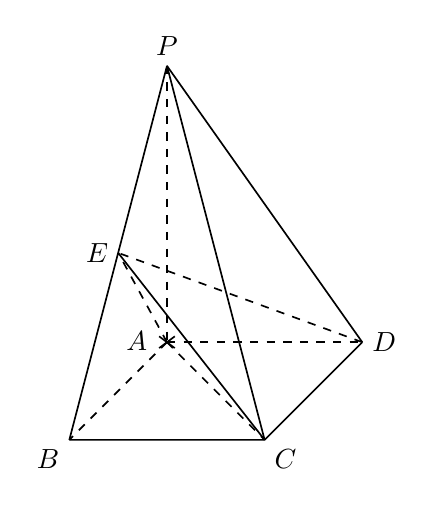
\begin{tikzpicture}[scale=0.62, semithick]
  \coordinate (B) at (0,0);
  \coordinate (C) at (4,0);
  \coordinate (A) at (2,2);
  \coordinate (D) at (6,2);
  \coordinate (P) at (2,7.66);
  \coordinate (E) at (1,3.83);

  % 可见棱
  \draw (B) -- (C) -- (D);
  \draw (P) -- (B);
  \draw (P) -- (C);
  \draw (P) -- (D);
  \draw (C) -- (E);

  % 被遮挡的棱
  \draw[dashed] (P) -- (A);
  \draw[dashed] (A) -- (B);
  \draw[dashed] (A) -- (D);
  \draw[dashed] (A) -- (C);
  \draw[dashed] (A) -- (E);
  \draw[dashed] (D) -- (E);

  % 原页在 A 处的遮挡叉号
  \draw[line width=0.6pt] (1.84,1.88) -- (2.16,2.12);
  \draw[line width=0.6pt] (1.84,2.12) -- (2.16,1.88);

  \node[above]       at (P) {$P$};
  \node[left]        at (E) {$E$};
  \node at (1.38,2.02) {$A$};
  \node[below left]  at (B) {$B$};
  \node[below right] at (C) {$C$};
  \node[right]       at (D) {$D$};
\end{tikzpicture}
